% Copyright 2007 by Marco Barisione
% Copyright 2011 by Henricus Bouwmeester
%
% This file may be distributed and/or modified
%
% 1. under the LaTeX Project Public License and/or
% 2. under the GNU Public License.
%
% If you want to specifically use the Helvetica Neue font which is the 
% font defined in the Branding and Identity Standards for UC Denver,
% you will need to use xelatex to compile as well as commenting out 
% the current font commands in the preamble then uncomment the fontspec
% package as well as the fontspec command after \begin{document}

\documentclass[10pt]{beamer}
\usefonttheme{serif}
% \documentclass[10pt,hyperref={pdfpagelabels=false}]{beamer}
\usepackage{amsmath,amsfonts,mathrsfs}
\usepackage{colortbl}

\newcommand\blfootnote[1]{%
  \begingroup
  \renewcommand\thefootnote{}\footnote{#1}%
  \addtocounter{footnote}{-1}%
  \endgroup
}

\newcommand{\etal}{{\it et al.\ }}
\newcommand{\bs}[1]{\boldsymbol{#1}}

\makeatletter
\renewcommand{\@makefnmark}{\hbox{\textsuperscript{\tiny{\@thefnmark}}}}
\makeatother

% set font to Helvetica
%\usepackage[T1]{fontenc}
%\usepackage[scaled=0.92]{helvet}
%\renewcommand*\familydefault{\sfdefault} %% Only if the base font of the document is to be sans serif
% \usepackage{fontspec}

\newif\ifuseblack
% for black theme, this should be
%     \useblacktrue
% for the white theme, this should be
%     \useblackfalse
\useblacktrue

\usetheme[pageofpages=of,                    % String used between the current page and the
                                             % total page count.
          bullet=circle,                     % Use circles instead of squares for bullets.
          titleline=true,                    % Show a line below the frame title.
          showdate=true,                     % show the date on the title page
          alternativetitlepage=true,         % Use the fancy title page.
          %titlepagelogo=../images/culogo, % Logo for the first page.
          titlepagelogo=../images/CUAnschutz_c_clr, % Logo for the first page.
          % Logo for the header on first page.
          \ifuseblack
             headerlogo=../images/pubHealth_tt2_rgb_rv_tp,
          \else
             headerlogo=../images/csph_biostatistics,    % Logo for white background.
          \fi
          watermark=../images/watermark,               % Watermark used in every page.
          watermarkheight=50pt,              % Height of the watermark.
          watermarkheightmult=6,             % The watermark image is 6 times bigger
                                             % than watermarkheight.
          ]{UCDenver}

\ifuseblack
   \usecolortheme{ucdblack}
\else
   \usecolortheme{ucdwhite}
\fi

% ============================================================================ %
% Document info
% ============================================================================ %

\author{Peter E. DeWitt}
\title[Intro to Git]{Git: Distributed Version Control \\ {\small An
Introduction}}
\institute{
\includegraphics[height=1.2\fontcharht\font`\B]{../images/culogo} AMC $|$ CSPH $|$ Biostats}
\date{25 February 2015}

\logo{
\includegraphics[height=15pt]{../images/csph_biostatistics}}

% ============================================================================ %
% Document
% ============================================================================ %

\begin{document} 
  \watermarkoff

  \begin{frame}[t,plain]
    \titlepage
  \end{frame}

  \begin{frame}[t]
    \frametitle{Outline}
    \framesubtitle{Why? and little bit of How?}
    \tableofcontents[hideallsubsections] 
  \end{frame}

    \section{Welcome: Why Git?}
  \begin{frame}[t]{Acknowledgements and Other Resources}

    \begin{itemize}
      \item Primary website: \url{http://git-scm.com}
      \item The first part of this presentation was inspired by, and copies
        from, `Git and
        Github\footnote{\url{github.com/rstudio/webinars/blob/master/2015-02/git-github.pdf}},' a webinar presented by Hadley Wickham.
      \item {\bf FREE} book: {\it Pro Git} 2nd
        edition\footnote{\url{http://git-scm.com/book/en/v2}}, best possible
        single source reference.
      \item This presentation highlights the first three chapters from
        {\it Pro Git}.
      \item A branching model I subscribe to:
        \url{http://nvie.com/posts/a-successful-git-branching-model/}

      \item Learn Git in 15 minutes: 
        \url{https://try.github.io/levels/1/challenges/1}
      \item A Simple guide and cheat sheet: 
        \url{http://rogerdudler.github.io/git-guide/}
      \item Git Videos: \url{http://git-scm.com/videos}

    \end{itemize} 
  \end{frame}

  \begin{frame}[t]
    \frametitle{Git}
    \begin{itemize}
      \item Can be difficult and frustrating to learn.
      \item Can be incorportated into your workflow.
      \item Your workflow may improve as you adapt to the git paradigm.
      \item Part of reproducable reporting.
      \item Payoffs: {\bf Safety} and {\bf Community}.
      \item Works okay for binary files 
        \begin{itemize} \item .docx, .pdf, .xlsx, \ldots \end{itemize}
      \item Works very, very, very, well for flat files: 
        \begin{itemize} \item .sas, .tex, .md, .txt, .R, .Rnw, .Rmd, .html, .c,
          .cpp, .js, .java, .csv, .dat, \ldots \end{itemize}
        
    \end{itemize}
    ``Failures, repeated failures, are finger posts on the road to achievement.
    One fails forward towards success.'' -- C.S.\ Lewis
  \end{frame}

  \begin{frame}[t]{A Story in Pictures} 
    \begin{center}
      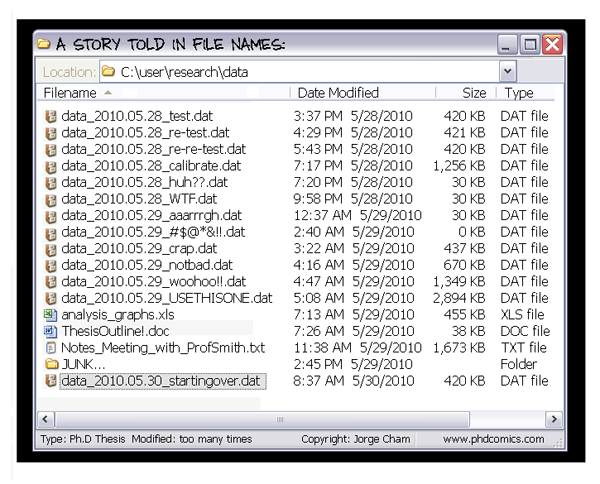
\includegraphics[height=2.350in]{../images/phd052810s.png} 
    \end{center} 
    \blfootnote{\url{http://www.phdcomics.com/comics/archive.php?comicid=1323}}
  \end{frame}
    

  \begin{frame}[t]{A Story in Pictures} 
    \begin{center}
      
\includegraphics[height=2.350in]{../images/phd101212s.png} 
    \end{center} 
    \blfootnote{\url{http://www.phdcomics.com/comics/archive.php?comicid=1531}}
  \end{frame}


  \begin{frame}[t]{A Story in Pictures} 
    \begin{center}
      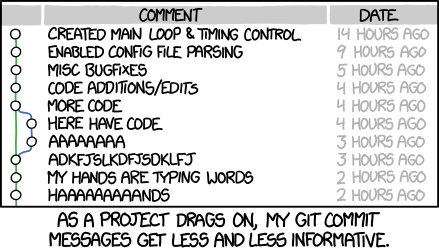
\includegraphics[height=2.000in]{../images/xkcd_git_commit.png} 
    \end{center} 
    \blfootnote{\url{http://xkcd.com/1296/}} 
  \end{frame}


  \begin{frame}[t]
    \frametitle{Changes}
    The history of a project can be viewed as a series of changes:
    \begin{center}
      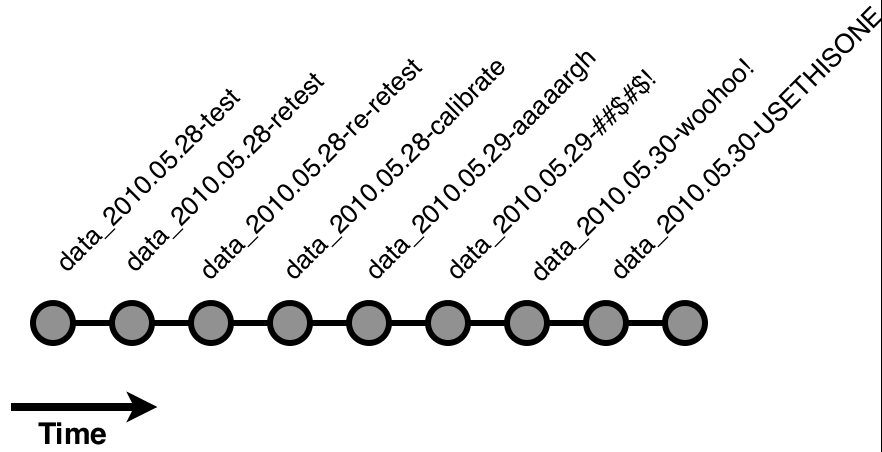
\includegraphics[height=2.00in]{../images/from-wickham-01.png} 
    \end{center} 
  \end{frame}

  \begin{frame}[t]
    \frametitle{Changes}
    \begin{itemize}
      \item A unique identifier
      \item What changed?
      \item When did it change?
      \item Who changed it?
      \item Why did it change?
      \item[]
      \item Difficult to coordinate with multiple files
    \end{itemize}
  \end{frame}

  \begin{frame}[t]
    \frametitle{Changes}
    With git, each change ({\bf commit}) is given a unique identifier, a {\bf
    sha}.
    \begin{center}
      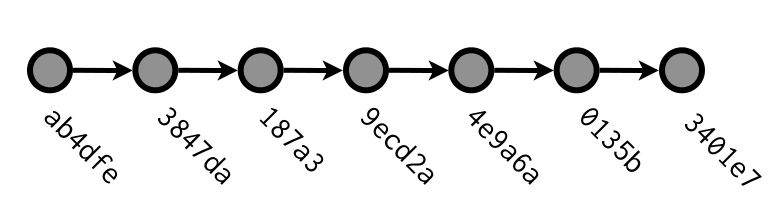
\includegraphics[width=0.98\textwidth]{../images/from-wickham-02.png} 
    \end{center} 

    \begin{itemize} 
      \item sha is a 40 digit long hexadecimal value.
        % $> 1.46 \times 10^{48}$ unique values
      \item sha is a key into a database that provides the author, date, and a
        description of the changes.
    \end{itemize} 
  \end{frame}

  \begin{frame}[t]
    \frametitle{Changes}
    You can also name individual commits.
    \begin{center}
      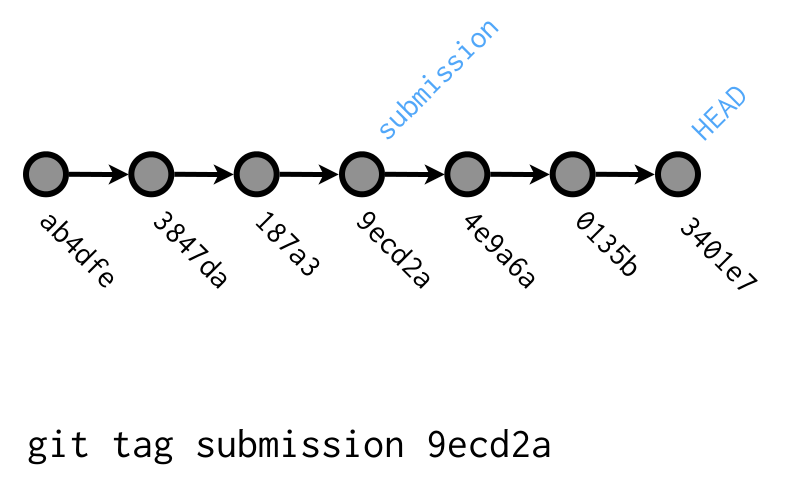
\includegraphics[height=2.00in]{../images/from-wickham-03.png} 
    \end{center} 

    \begin{itemize} 
      \item {\tt HEAD} is the location the working directory is set to.
      \item {\tt submission} is an example of a {\bf tag}
    \end{itemize} 
  \end{frame}

  \begin{frame}[t]
    \frametitle{Changes}
    Then see exactly what was changed 
    \begin{center}
      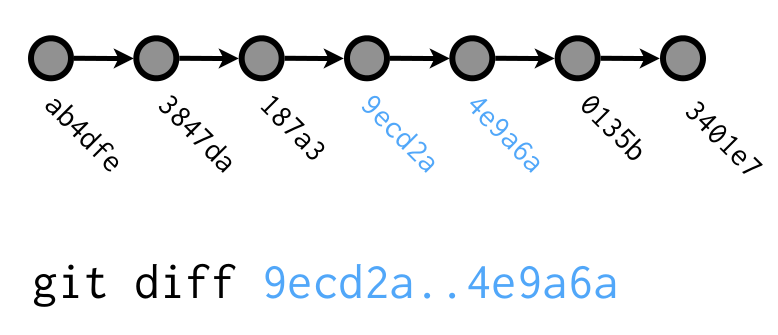
\includegraphics[height=2.00in]{../images/from-wickham-04.png} 
    \end{center} 
  \end{frame}

  \begin{frame}[t]
    \frametitle{Changes}
    You can revert to a previous change with git checkout
    \begin{center}
      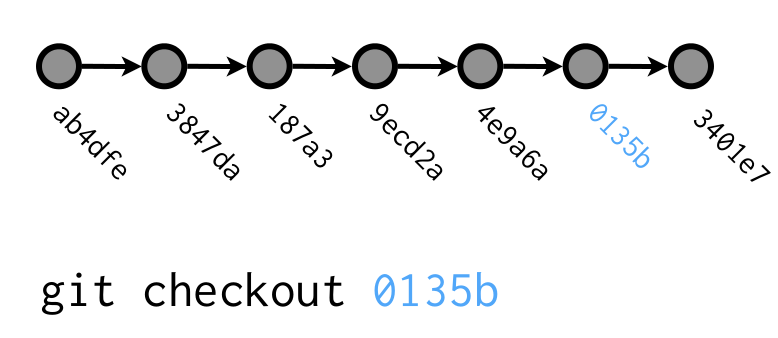
\includegraphics[height=2.00in]{../images/from-wickham-05.png} 
    \end{center} 
  \end{frame}

  \begin{frame}[t]
    \frametitle{Changes}
    That allows you to undo mistakes
    \begin{center}
      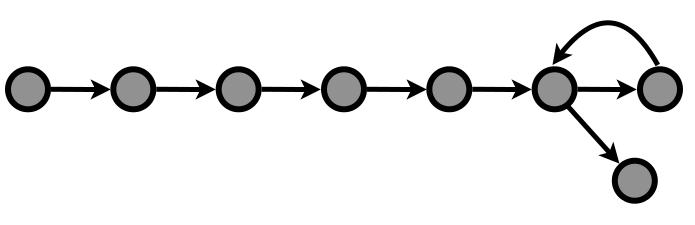
\includegraphics[width=0.98\textwidth]{../images/from-wickham-06.png} 
    \end{center} 
  \end{frame}
 
  \section{Getting Started}

\begin{frame}[t]{A summary of Chapter 1 from {\it Pro Git}}
  \begin{itemize}
    \item Version control paradigms.
    \item What is Git?
    \item How does Git work?
    \item[]
    \item How to use Git will be discussed in the next section.
  \end{itemize}
\end{frame}

\subsection{About Version Control}
\begin{frame}[t]{Local Version Control System}
  \begin{center}
    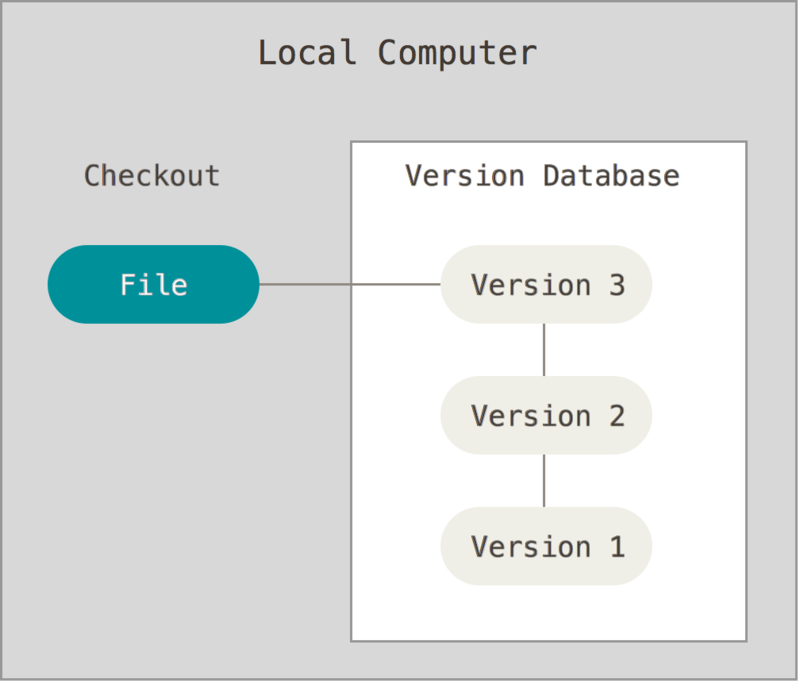
\includegraphics[height=2.75in]{../images/02-getting-started/local}
  \end{center}
\end{frame}

\begin{frame}[t]{Centralized Version Control Systems}
  \begin{center}
    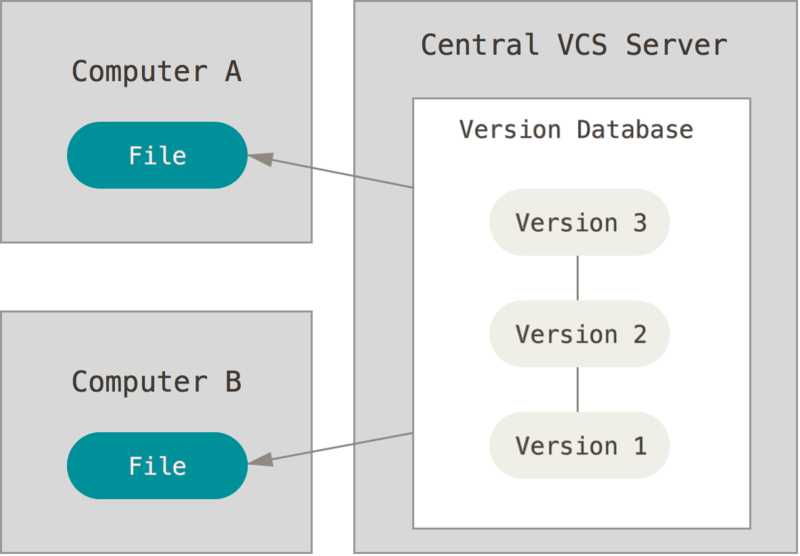
\includegraphics[height=2.75in]{../images/02-getting-started/centralized}
  \end{center}
\end{frame}

\begin{frame}[t]{Distributed Version Control Systems}
  \begin{center}
    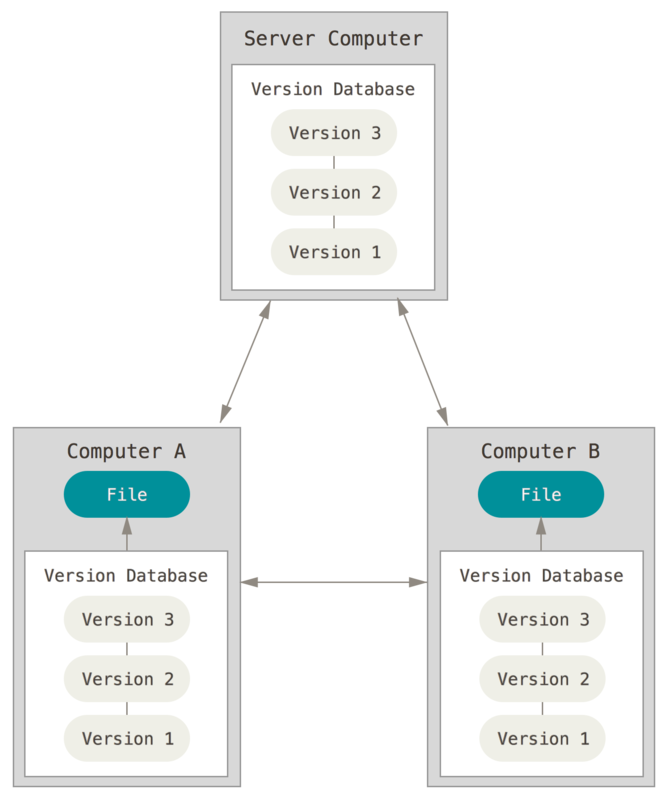
\includegraphics[height=2.75in]{../images/02-getting-started/distributed}
  \end{center}
\end{frame}

\subsection{A Short History of Git}
\begin{frame}[t]{Short History of Git}
  \begin{itemize}
    \item Linux (Linus Torvalds) vs BitKeeper
    \item 2005: Linux development community sets out to develop their own DVCS
      with goals for the new system of
      \begin{itemize}
        \item speed,
        \item simple design,
        \item strong support for non-linear development (thousands of parallel
          branches),
        \item fully distributed, and
        \item albe to handle large projects, like the Linux kernel,
          efficiently.
      \end{itemize}
  \end{itemize}
\end{frame}

\subsection{Git Basics}
\begin{frame}[t,allowframebreaks]{Snapshots, Not Differences}

  The Subversion model: file-based changes.

  \begin{center}
    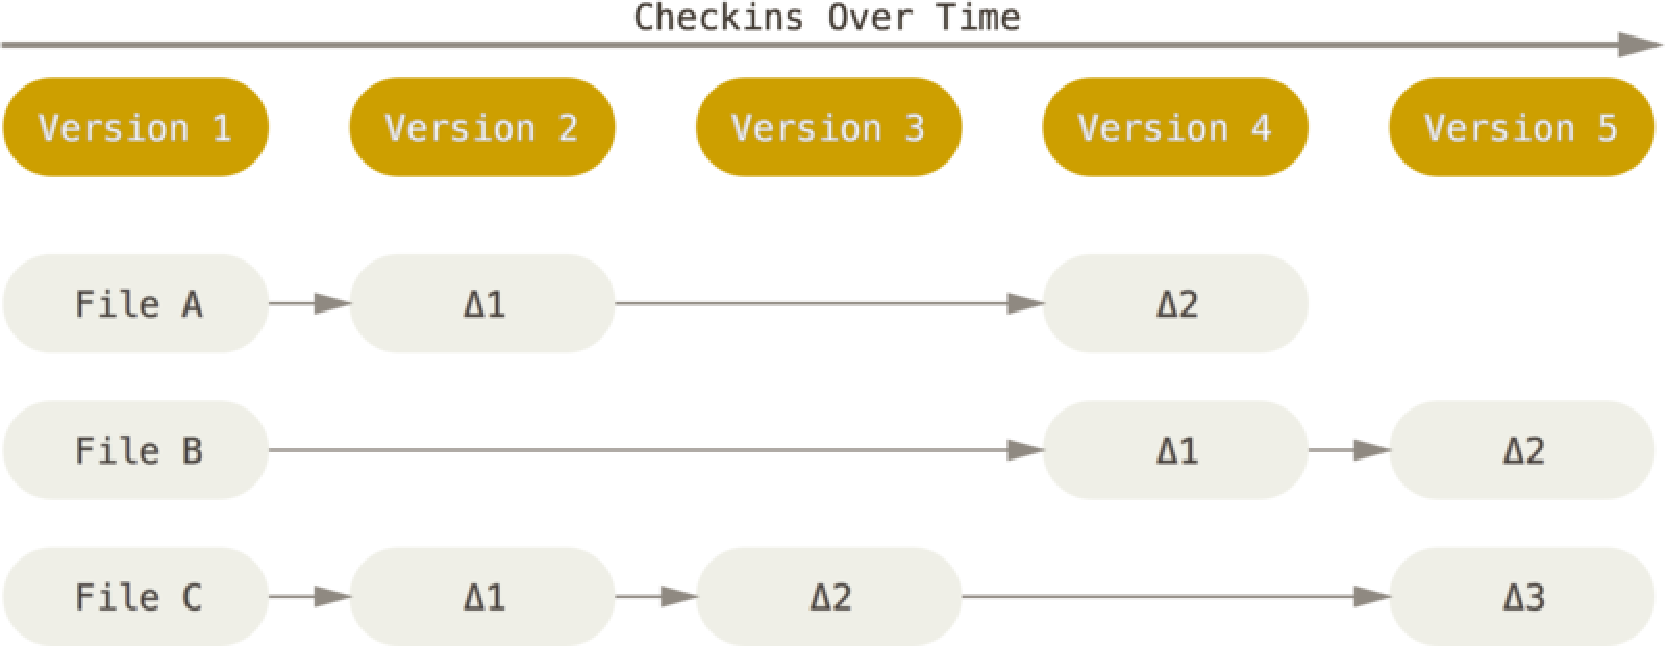
\includegraphics[width=0.98\textwidth]{../images/02-getting-started/deltas}
  \end{center}

  \pagebreak

  The Git model: a stream of snapshots.

  \begin{center}
    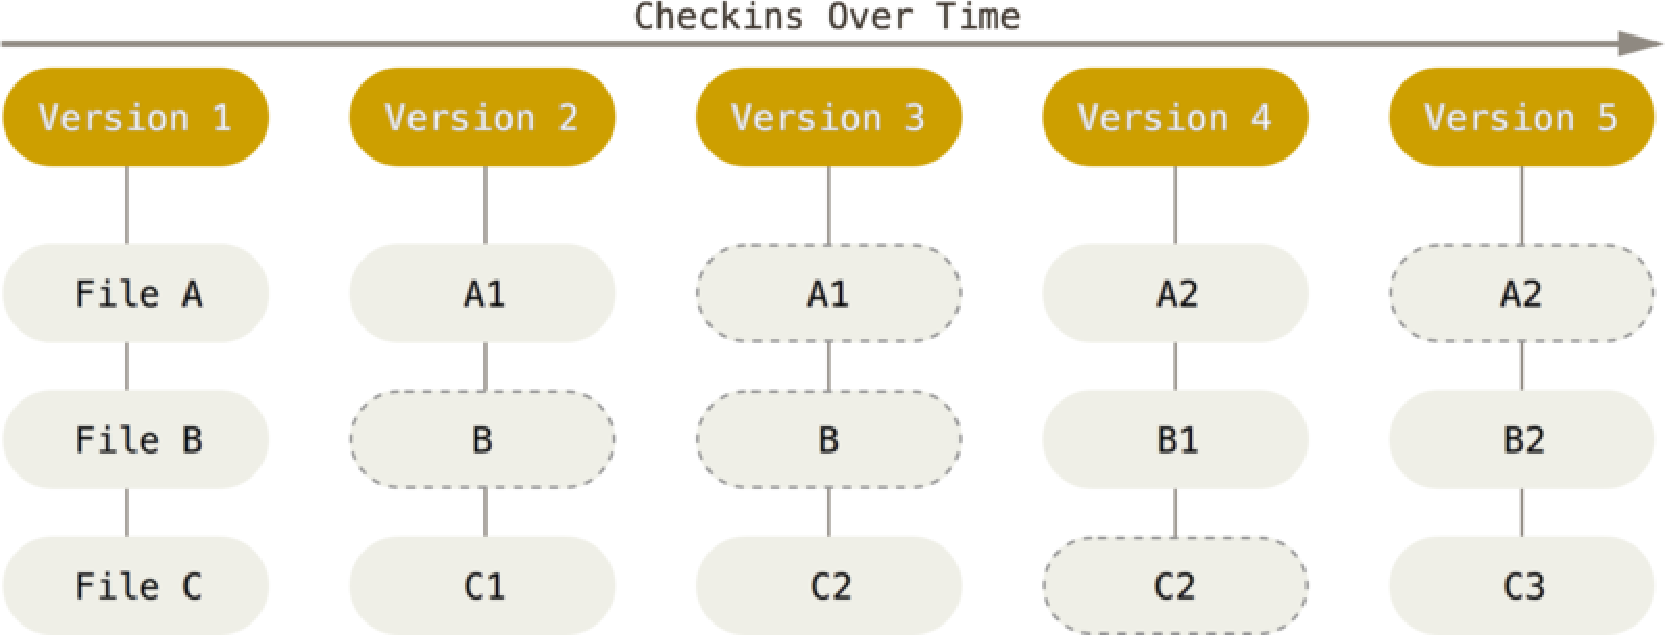
\includegraphics[width=0.98\textwidth]{../images/02-getting-started/snapshots}
  \end{center}

\end{frame}

\begin{frame}[t]{Nearly Every Operation is Local}
  \begin{itemize}
    \item Most operations are local.
      \begin{itemize}
        \item No need to talk to other computers on a network.
        \item The entire project history is on your local disk.
      \end{itemize}

    \item You can work offline.
    \item You can work off VPN.  
  \end{itemize}
\end{frame}

\begin{frame}[t]{Git Has Integrity}
  \begin{itemize}
    \item Everything is check-summed (remember the sha?)
    \item You can't lose informatin in transit nor get a file corruption without
      Git being able to detect it.
    \item Git stores everything in its database not by file name but by the hash
      value of its contents.
  \end{itemize}
\end{frame}

\begin{frame}[t]{Git Generally Only Adds Data}
  \begin{itemize}
    \item Nearly all actions in Git add data to the Git database.
    \item It is difficult to do anything that is not undoable.
    \item You can lose/corupt un-committed changes.
    \item It is very difficult to lose anything after a commit, especially with
      frequent pushes to other repositories.
  \end{itemize}
\end{frame}

\begin{frame}[t,allowframebreaks]{The Three States}
  This is the main thing to remember about Git if you want the rest of your
  learning process to go smoothly.  Git has three main states that files reside
  in.

  \begin{enumerate}
    \item Committed
      \begin{itemize}
        \item data is safely stored in the local database.
      \end{itemize}
    \item Modified
      \begin{itemize}
        \item changed the file(s) but have not committed to the database yet.
      \end{itemize}
    \item Staged
      \begin{itemize}
        \item Marked modified file(s) in its current version to go into the next
          commit snapshot.
      \end{itemize}
  \end{enumerate}

  This leads to three main sections of a Git project:
  \begin{enumerate}
    \item the Git directory,
    \item the working directory, and
    \item the staging area.
  \end{enumerate}

  \pagebreak

  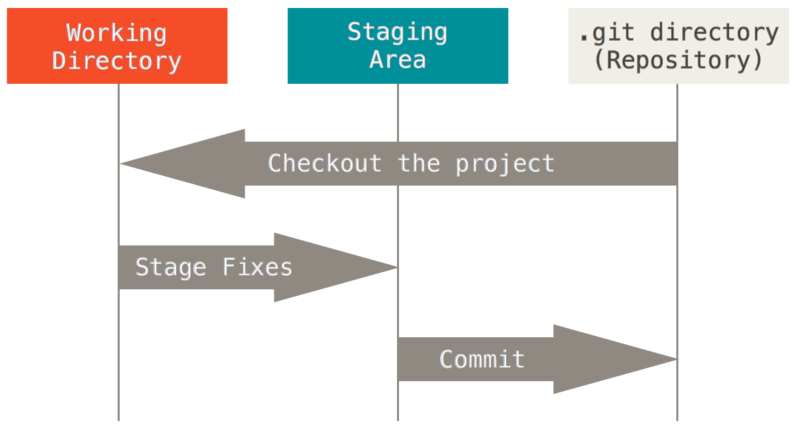
\includegraphics[height=1.0in]{../images/02-getting-started/areas.png}

  Basic Git workflow:
  \begin{enumerate}
    \item Modify files in working directory.
    \item Stage files, adding snapshots of them to staging area.
    \item Commit.  Takes the files as they are in the staging area and stores
      that snapshot permanently in your Git directory.
  \end{enumerate} 
\end{frame}

\subsection{The Command Line}
\begin{frame}[t]{Different ways to use Git}
  \begin{itemize}
    \item Original command line tools.
    \item Many graphical user interfaces (GUIs) with verying capabilities.

    \item Command line allows you to use {\bf all} Git commands.
    \item GUIs allow for only a subset of Git commands.

    \item After install, on Windows, Mac OSx, or Linux, command line will be
      available.
    \item GUIs, take your pick. \url{http://git-scm.com/downloads/guis} has 12
      differnt GUIs with different features, OS requirments, \ldots, surely
      dozens of others exist too.
  \end{itemize}
\end{frame}

\subsection{Intalling Git}
\begin{frame}[t]{Git is Free!}
  \begin{itemize}
    \item Linux: install via {\tt yum install git} or {\tt apt-get install git}.
    \item Mac: Xcode Command Lines Tools.
    \item Windows: \url{http://git-scm.com/download/win}
    \item Install form source too, if you want.
  \end{itemize}
\end{frame}

\begin{frame}[t]{Set up}
  Need to run this once after install.  Done via command line, can be done in
  {\it some} GUIs.

  {\tt
    \$ git config --global user.name "Peter DeWitt"

    \$ git config --global user.email "peter.dewitt@ucdenver.edu" 
  } 
\end{frame}

\begin{frame}[t]{Getting Help}
  You can get information on Git verbs via:

  {\tt
    \$ git help $<$verb$>$

    \$ git $<$verb$>$ --help

    \$ man git-$<$verb$>$ 
  } 
\end{frame}

  \section{Basic Git Use}
\begin{frame}[t]
  \frametitle{Outline}
  \framesubtitle{Why? and little bit of How?}
  \tableofcontents[currentsection,hideallsubsections] 
\end{frame}

\begin{frame}[t]{What will be covered in this section?}
  \begin{itemize}
    \item Working on a local repository.
    \item Working with a remote.
    \item Working with other people with a common remote.
    \item[]
    \item Read Chapter 2 of {\it Pro Git} for more information.
    \item[]
    \item Examples will be done using the command line.
  \end{itemize}
\end{frame}


\begin{frame}[t]
  \frametitle{Working on a Local Repository}
  \framesubtitle{Objectives:}
    We will learn the following Git verbs:
  \begin{itemize}
    \item {\tt init}
    \item {\tt status}
    \item {\tt add}
    \item {\tt commit}
    \item {\tt diff}
    \item {\tt log}
    \item {\tt checkout} 
    %\item {\tt reset}
    \item {\tt mv} 
    \item {\tt rm}
  \end{itemize}
  
  Other helpful things:
  \begin{itemize}
    \item {\tt .gitignore} files
  \end{itemize}
\end{frame}

\begin{frame}[t]
  \frametitle{Working with a Remote}
  \framesubtitle{Objectives:}
  Remote Hosting Options
  \begin{itemize}
    \item \url{github.com}, \url{bitbucket.com}, and many others.
    \item Read the end user agreements. 
    \item Public or Private repo: data is stored on a public server.
    \item In my office is a git server, cbcgit.ucdenver.pvt.  If you want an
      account on this machine send me an email and I'll set you up.
  \end{itemize}

  Authentication:
  \begin{itemize}
    \item https
    \item ssh
  \end{itemize}

  We will learn the following Git verbs:
  \begin{itemize}
    \item {\tt remote}
    \item {\tt push}
    %\item {\tt pull}
    \item {\tt clone}
    \item {\tt fetch}
    \item {\tt merge}
  \end{itemize} 
\end{frame}

\begin{frame}[t]{Objectives:}
  \frametitle{Working with Others and Remotes}
  Owners of the repo can set read/write permissions.

  We will learn the following Git verbs:
  \begin{itemize}
    \item {\tt merge}
    \item {\tt diff-tools}
  \end{itemize} 
\end{frame}


  \section{Branching}

\begin{frame}[t]
  \frametitle{Outline}
  \framesubtitle{Why? and little bit of How?}
  \tableofcontents[currentsection,hideallsubsections] 
\end{frame}

\begin{frame}[t]{What will be covered in this section?}
  \begin{itemize}
    \item Why Branching?
    \item How to Branch.
    \item[]
    \item Read Chapter 3 of {\it Pro Git} for more information.
    \item[]
    \item Branching and merging are fundamental to the use of Git.  
      \begin{itemize}
        \item In other VC software system branching and merging are either
          imposible or very, very difficult.
        \item Git makes it easy!
      \end{itemize}

    \item I'm hoping to have time to talk about this, but I expect to have run
      out of time.  It's okay, working on just the master branch for now is a
      good starting place.  Learn all the verbs needed to work on one branch and
      then the details to learn branching will come as a natural next step.
  \end{itemize}
\end{frame}

\begin{frame}[t]
  \frametitle{Why is Branch?}
  \begin{itemize}
    \item Develpment off of the master branch.
    \item Work in a sandbox for features.
    \item What's down this rabit hole?
    \item[]
    \item ``I've got this great idea!  Wait, \#$@$!!?\%, it's not going
      anywhere.  Well, maybe?  I'd done know.'' $\leftarrow$ Make a branch! :)
  \end{itemize}
\end{frame}

\begin{frame}[t]{}
  \frametitle{Branching Model}
  \framesubtitle{ \url{http://nvie.com/posts/a-successful-git-branching-model/} }

  \begin{center} 
    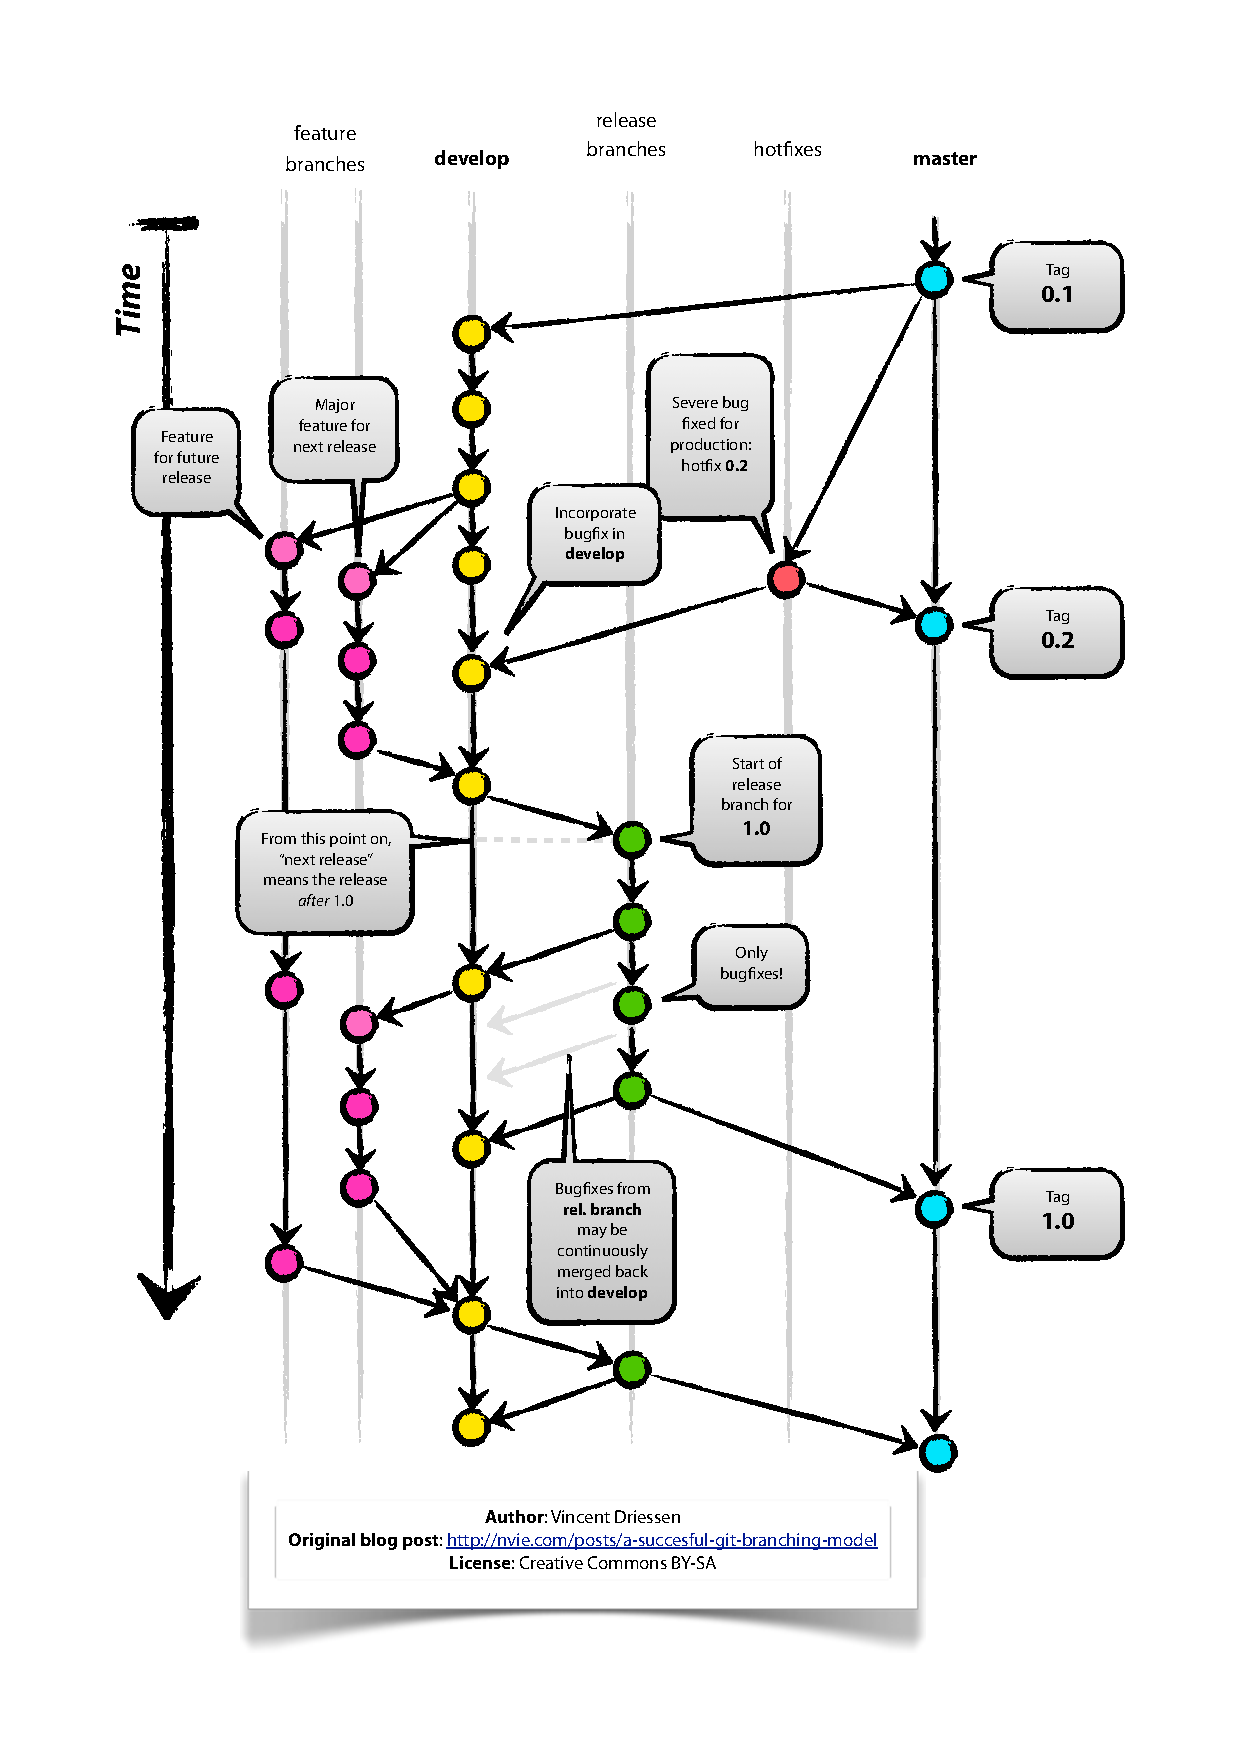
\includegraphics[height=2.75in]{../images/Git-branching-model}
  \end{center}
\end{frame}


% \subsection{Branches in a Nutshell}
% \begin{frame}[t]{}
% \end{frame}
% 
% \subsection{Basic Branching and Merging}
% \begin{frame}[t]{}
% \end{frame}
% 
% \subsection{Branch Management}
% \begin{frame}[t]{}
% \end{frame}
% 
% \subsection{Branching Workflows}
% \begin{frame}[t]{}
% \end{frame}
% 
% \subsection{Remote Branches}
% \begin{frame}[t]{}
% \end{frame}
% 
% \subsection{Rebasing}
% \begin{frame}[t]{}
% \end{frame}
% 
% \begin{frame}[t]{}
% \end{frame}
% 
% 



  \section{Closing}
  \begin{frame}[t]{Outline}
    \tableofcontents[currentsection,hideallsubsections]
  \end{frame}

  \begin{frame}[t] 
    \frametitle{Closing}
    \begin{center}
    Thank you for your time.

    \vspace{1in}

    The floor is open for questions and comments.
    \end{center} 
  \end{frame}

\end{document}

